% Options for packages loaded elsewhere
\PassOptionsToPackage{unicode}{hyperref}
\PassOptionsToPackage{hyphens}{url}
%
\documentclass[
  12pt,
]{article}
\usepackage{lmodern}
\usepackage{amssymb,amsmath}
\usepackage{ifxetex,ifluatex}
\ifnum 0\ifxetex 1\fi\ifluatex 1\fi=0 % if pdftex
  \usepackage[T1]{fontenc}
  \usepackage[utf8]{inputenc}
  \usepackage{textcomp} % provide euro and other symbols
\else % if luatex or xetex
  \usepackage{unicode-math}
  \defaultfontfeatures{Scale=MatchLowercase}
  \defaultfontfeatures[\rmfamily]{Ligatures=TeX,Scale=1}
\fi
% Use upquote if available, for straight quotes in verbatim environments
\IfFileExists{upquote.sty}{\usepackage{upquote}}{}
\IfFileExists{microtype.sty}{% use microtype if available
  \usepackage[]{microtype}
  \UseMicrotypeSet[protrusion]{basicmath} % disable protrusion for tt fonts
}{}
\usepackage{xcolor}
\IfFileExists{xurl.sty}{\usepackage{xurl}}{} % add URL line breaks if available
\IfFileExists{bookmark.sty}{\usepackage{bookmark}}{\usepackage{hyperref}}
\hypersetup{
  pdftitle={Quantile Regression Analysis for Statin Effects on Body mass Index},
  pdfkeywords={My keywords},
  hidelinks,
  pdfcreator={LaTeX via pandoc}}
\urlstyle{same} % disable monospaced font for URLs
\usepackage[margin=1in]{geometry}
\usepackage{longtable,booktabs}
% Correct order of tables after \paragraph or \subparagraph
\usepackage{etoolbox}
\makeatletter
\patchcmd\longtable{\par}{\if@noskipsec\mbox{}\fi\par}{}{}
\makeatother
% Allow footnotes in longtable head/foot
\IfFileExists{footnotehyper.sty}{\usepackage{footnotehyper}}{\usepackage{footnote}}
\makesavenoteenv{longtable}
\usepackage{graphicx,grffile}
\makeatletter
\def\maxwidth{\ifdim\Gin@nat@width>\linewidth\linewidth\else\Gin@nat@width\fi}
\def\maxheight{\ifdim\Gin@nat@height>\textheight\textheight\else\Gin@nat@height\fi}
\makeatother
% Scale images if necessary, so that they will not overflow the page
% margins by default, and it is still possible to overwrite the defaults
% using explicit options in \includegraphics[width, height, ...]{}
\setkeys{Gin}{width=\maxwidth,height=\maxheight,keepaspectratio}
% Set default figure placement to htbp
\makeatletter
\def\fps@figure{htbp}
\makeatother
\setlength{\emergencystretch}{3em} % prevent overfull lines
\providecommand{\tightlist}{%
  \setlength{\itemsep}{0pt}\setlength{\parskip}{0pt}}
\setcounter{secnumdepth}{5}
\usepackage{setspace}\doublespacing
\usepackage{float}

\title{Quantile Regression Analysis for Statin Effects on Body mass Index}
\author{}
\date{\vspace{-2.5em}April 22, 2021}

\begin{document}
\maketitle
\begin{abstract}
My abstract
\end{abstract}

{
\setcounter{tocdepth}{2}
\tableofcontents
}
\section{introduction}

High BMI has negative impact on public health. Due to high cost of obesity, it is crucial to get better understanding of the underlying risk factor for obesity. This can help decision makers to create a new regulation that help to prevent and to stop the dramatic increase in the BMI index.

Body Mass Index (BMI) plays an important role in predicting heart disease risk(Katzmarzyk et al. 2012). Approximately, 18 million deaths annually per year are caused by cardiovascular diseases(CVD), and similar to this number of nonfatal cardiovascular events (Hay et al. 2017).
In 2011, annual costs for CVD and stroke were \(\$320.1\) billion, which is more than cancer cost. This cost includes \$195.6 billion in direct costs (healthcare costs), and the cost of future productivity loss is \$124.5 (Mozaffarian et al. 2015). Important factors associated with CVD are high body mass index (BMI) and abnormal lipid ratio (Yusuf et al. 2004), (Anderson et al. 1991). Lowering low-density lipoprotein (LDL) by using statin or other drugs reduces the risk of cardiovascular diseases even with a population with no CVD (Yusuf et al. 2016). Ferrieres et al.~(Ferrières et al. 2018) studied the effect of BMI on the choice of lipid-lowering treatment. It is been found that statin intensity increases with the high level of BMI(\(\rho=0.13\)).
\begin{equation}
y_{i}=  
 \left\{
\begin{array}{ll}
 \beta_{01}+\beta_{11}x_i+\beta_{21}x_i^2+ \beta_{31}x_i^3+\eps_i & \mbox{if } x_i< c \\
 \beta_{02} & \mbox{if } x_i \geq c
\end{array}
\right.
\end{equation}
Taking cholesterol drug medication associates with a high risk of elevating BMI level. It is been shown that statin users consume 192 additional calories per day which causes gaining a 6 lb to 11 lb. in a year. Statin users gain 1.3 units in the BMI measure while non-staining users gain 0.4 unit. Moreover, consumption of fat in statin users raised by 14.4\%(Sugiyama et al. 2014).

Logistic regression helps us to find out the group that has a higher odd of obesity, and ordinary least squares (OLS) regression helps us to study the effects of predictors on the average mean of the response. For example, estimating the association of different factors like a lipid-lowering drug with the conditional mean of BMI using OLS or logistic regression model(Ferrières et al. 2018). Both of these approaches do not give us insight into the predictor's effects on different quantiles of the responses.

Quantile regression is used to investigate the heterogeneity in the association of the \(\tau\)th quantile of BMI with a set of independent predictors, that is investigate the effects of a specific predictors on the various quantiles of the BMI. BMI departs normality because of the skewness on the right and left tails (Flegal 1999). Estimation of underweight and overweight can be affected by the violation of normality. Quantile regression is a crucial tool used to estimate BMI with the dispersion of the association with predictors.

Quantile regression has many successful applications in ecology where different factors interact in a complicated way that produces different variations of one factor for different levels of another variable (Cade and Noon 2003). The association between BMI and the set of predictors; low childhood socioeconomic position, high maternal weight, low childhood general cognition is stronger in the upper end of BMI quantile. This trend is found in the UK population(Bann, Fitzsimons, and Johnson 2020). One cause of this heterogeneity is that risk factors may have stronger effect on patients with worse health, and these effects may diminishes when conditional mean of the BMI is studied.

We found that spline regressions produce a different estimate than polynomial regressions. Polynomial regression using the quadratic term of predictors forces the response to take convex or concave shape, see Figure 1.12 (Koenker 2005). This is because the limit of quadratic functions approach \(\pm\infty\) as \(x\rightarrow\pm\infty.\) However, when we model the predictor as splines the response is not forced to take a specific shape. In the latter case, different polynomials are constructed for the different regions in the range of predictors.

\section{Quantile Regression}

Quantile regression is a tool used to regress the dependent variable with high variance over the independent variables. QR is developed to study the relationships between variables that have week or no-relationships between their means. One of the advantages of using QR over OLS is QR is robust for outliers.

For a random variable \(X\), the cumulative distribution function (CDF) is \[F(X)=P(X\leq x),\] and the \(\tau\)th quantile of \(X\) is defined by \[ F^{-1}(\tau)=\text{inf}\{x: F(x)\ge \tau\} \] where \(0<\tau<1\).
Let the loss function is defined by \[\rho_{\tau}(u)= u(\tau-I_{(u<0)})\] where \(I\) is the indicator function (Koenker 2005). The quantile estimator is the value that minimizes the expected loss function

\[E\rho_{\tau}(X-\hat{x})=(\tau-1)\int_{-\infty}^{\hat{x}} (x-\hat{x})dF(x)+\tau\int_{\hat{x}}^{-\infty} (x-\hat{x})dF(x).\]
Differentiating with respect to \(\hat{x}\), we get
\[ 0  =(\tau-1)\int_{-\infty}^{\hat{x}} dF(x)+\tau\int_{\hat{x}}^{-\infty} dF(x)
=F(\hat{x})-\tau.\]
Due to the monotonicity of the cumulative distribution function, any solution that satisfies \(\{x:F(x)=\tau \}\) is a minimizing for the expected loss function.

Least square method expresses conditional mean of y given x as \(\mu(x)=x^T\beta\) and it solves \[ \underset{\beta\in \mathcal{R}^p}{\text{min}}\sum_{i=1}^n(y_i- x_i^T\beta)^2.\] Quantile regression expresses conditional quantile function \(Q_y(\tau|x)=x^T \beta ({\tau)}\) and solve \[ \underset{\beta\in \mathcal{R}^p}{\text{min}}\sum_{i=1}^n\rho_{\tau}(y_i- x_i^T\beta)^2.\]This minimization problem can be reformulated to a linear programming problem \[ \underset{\beta\in \mathcal{R}^p}{\text{min}} \]

\subsection{Quantile Regression Technique }

\subsection{splines}

A continuous predictor can be modeled as linear, say \(X\), or nonlinear term, say \(X^2\) depends on the relationship with the response variable. Most of the relations between the responses and predictors variables are complicated to the point that linear regressions are not suitable to model these relationships(Bruce, Bruce, and Gedeck 2020). For example, the response to different levels of drug doses is not a linear relationship. Linear regressions can be generalized to deal with nonlinear effects. One approach is through including polynomial terms in the regression equation. This approach is called Polynomial regression. The mathematical model for \(n\) degree polynomial regression is shown in the Eq\eqref{non}
\begin{equation}\label{non}
 y=\beta_0+\beta_1 X+\beta_2 X^2+\cdots+\beta_nX^n.
 \end{equation}

One of the limitations of using polynomial regression is the curvature that can be captured is limited with low order terms. However, including higher-order terms has a negative impact on the model by introducing undesirable ``wiggliness'' in the regression equation. Another robust approach to model nonlinear relationships is splines. It is similar to a technique used by draftsmen in plotting curves. The spline is a process of constructing a set of piece-wise continuous
polynomials that are smoothly connected at a set of points in the range of the predictor variable. The connection points are called knots i.e.~splines are used to smoothly interpolate between certain points. Let \(a,b\) ,and \(c\) are the endpoints of the \(x\)-axis intervals. A smooth cubic spline function is defined by the following equation.
\begin{equation}
f(X)=X\beta=\beta_{0}+\beta_{1}X+\beta_2X^2+\beta_{3}X^{3}+\beta_{4}(X-a)_{+}^3+\beta_{5}(X-b)_{+}^3+\beta_6(X-c)_{+}^3,
\end{equation}

where \[(u)_{+}=  
 \left\{
\begin{array}{ll}
u  & \mbox{if } u > 0 \\
0 & \mbox{if } u \leq 0
\end{array}
\right. \]

\section{Methods}

A multivariate quantile regression model is used to assess the characteristics of the association variability in different quantiles of the conditional distribution of the body mass index.

The independent variables in our model are gender, race, age, total cholesterol, cholesterol drug use (yes or no). All types of cholesterol drugs are used including statins. The included races are non-Hispanic white, non-Hispanic black, Hispanic, or other.

\section{Numerical Example}
\subsection{Data}

The data used in this study is National Health and Nutrition Examination Survey data (NHANES)(Disease Control and (CDC) 2018). The survey examines a nationally representative sample of the U.S. population. It focuses on a variety of health and nutrition measurements. The survey data are released every two years cycle. In this study, we accumulated 6 cycles of NHANES data (2007--2018). We used two data files: One contains demographic variables, such as age, sex, race, income, etc., and the other contains data that are related to body measurements, such as BMI, head circumference, etc. These files are merged by using the respondent sequence number (SEQN)
There are around 12,000 records. We selected a population age between 20 and 80.
BMI are classified into different categories according to underweight, 18.5 kg/m2; normal weight, 18.5 to 25 kg/m2; overweight, 25 to 30 kg/m2; obese, 30 to 35 kg/m2; and very obese more than 35 kg/m2.

\begin{longtable}[]{@{}lcr@{}}
\toprule
Syntax & Male & Female\tabularnewline
\midrule
\endhead
count & 5990 & 6416\tabularnewline
Mean of Age & 49.9 & 49.73\tabularnewline
BMI & 28.549 & 29.379\tabularnewline
TC & &\tabularnewline
Statin use (ratio) & 0.198 & 0.181\tabularnewline
\bottomrule
\end{longtable}

base\_box\_plot

\begin{figure}

{\centering 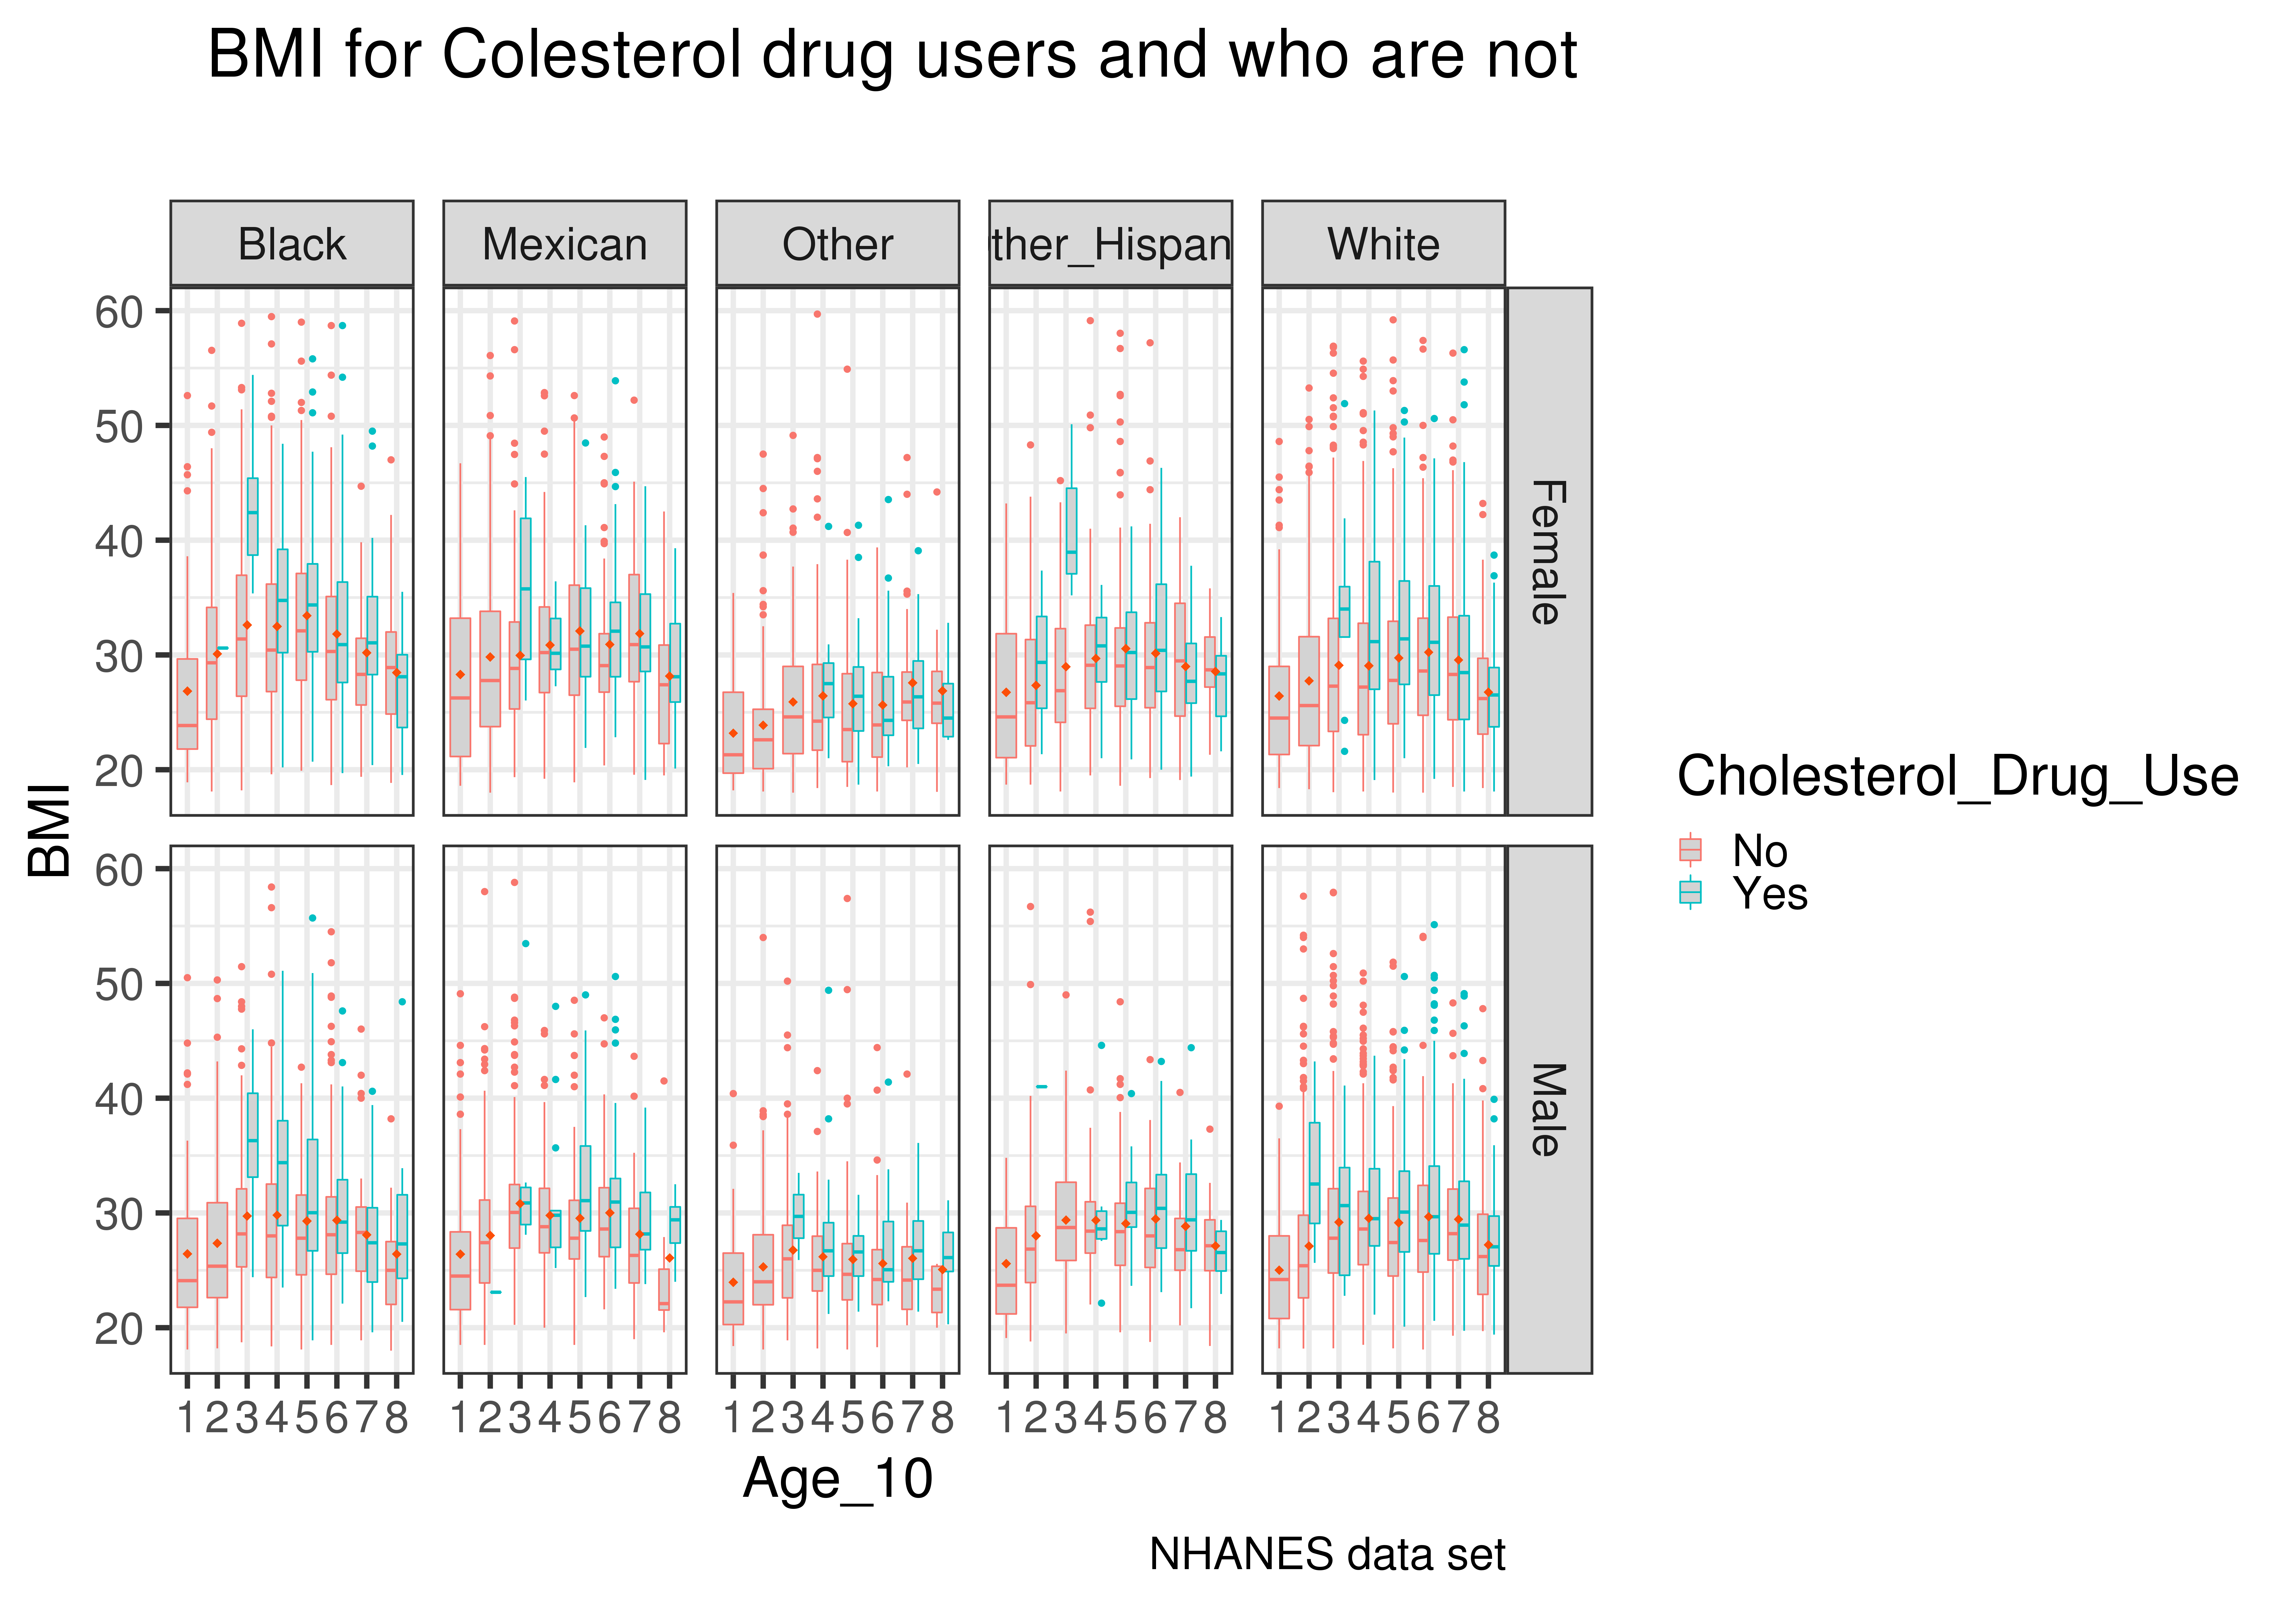
\includegraphics[width=1\linewidth]{/home/mabdulsa/BMI/images/base_box_plot} 

}

\caption{Illustration of data distribution using a box plot. The plot compares cholesterol drug users vs non-cholesterol drug users}\label{fig:box}
\end{figure}

Figure \ref{fig:box} shows the association between age and BMI with respect to cholesterol drug is inconsistent. At the early age, the correlation is positive while at the middle age the correlation is almost flat, and at the old age the correlation is negative. Moreover, at low age cholesterol medications are described only for a population with high BMI, but at a higher age, the difference in term of the BMI for a population that takes cholesterol medication and without cholesterol medication decreases until it diminishes as in the white population. The heterogeneity can also be seen in gender ?, for the Hispanic female population, the cholesterol medication is taken by the population with lower BMI if compared to the population that does not take cholesterol medication.

\begin{figure}

{\centering 
\includegraphics[width=0.8\linewidth]{/home/mabdulsa/BMI/images/exploratory} 

}

\caption{A better figure caption}\label{fig:data}
\end{figure}

\begin{figure}

{\centering 
\includegraphics[width=0.8\linewidth]{/home/mabdulsa/BMI/images/exploratory2} 

}

\caption{A better figure caption}\label{fig:unnamed-chunk-1}
\end{figure}

So,

\begin{figure}

{\centering 
\includegraphics[width=0.8\linewidth]{/home/mabdulsa/BMI/images/quant90} 

}

\caption{A 90th quantile of BMI ploted with repect to age. The population grouped with repect gender and fasting blood glucose level: prediabetes nad diabetes}\label{fig:unnamed-chunk-2}
\end{figure}

\section{Results}

The resulting estimate of effects on conditional mean of BMI level may not reflect the size and nature of these effects on lower or upper quantile. For example, in Figure \ref{fig:resu1}, the conditional mean effect of gender on BMI level is about -1, that is on average male's BMI is less than a female's BMI by one unit. However, the disparity of the gender effects on lower tails is much larger which is about 1, but the disparity is lower for the upper tail of the distribution somewhat around -3 unit.

From the OLS it is obvious cholesterol drug users have on average higher BMI levels if compared to non-cholesterol drug users which are around 1.75. The disparity in BMI level for cholesterol drug users vs non-cholesterol drug users is almost the same for different Quantiles. cholesterol drug use seems to be associated with rather large effects on BMI levels somewhat around 1.5 to 1.7.

\begin{figure}

{\centering 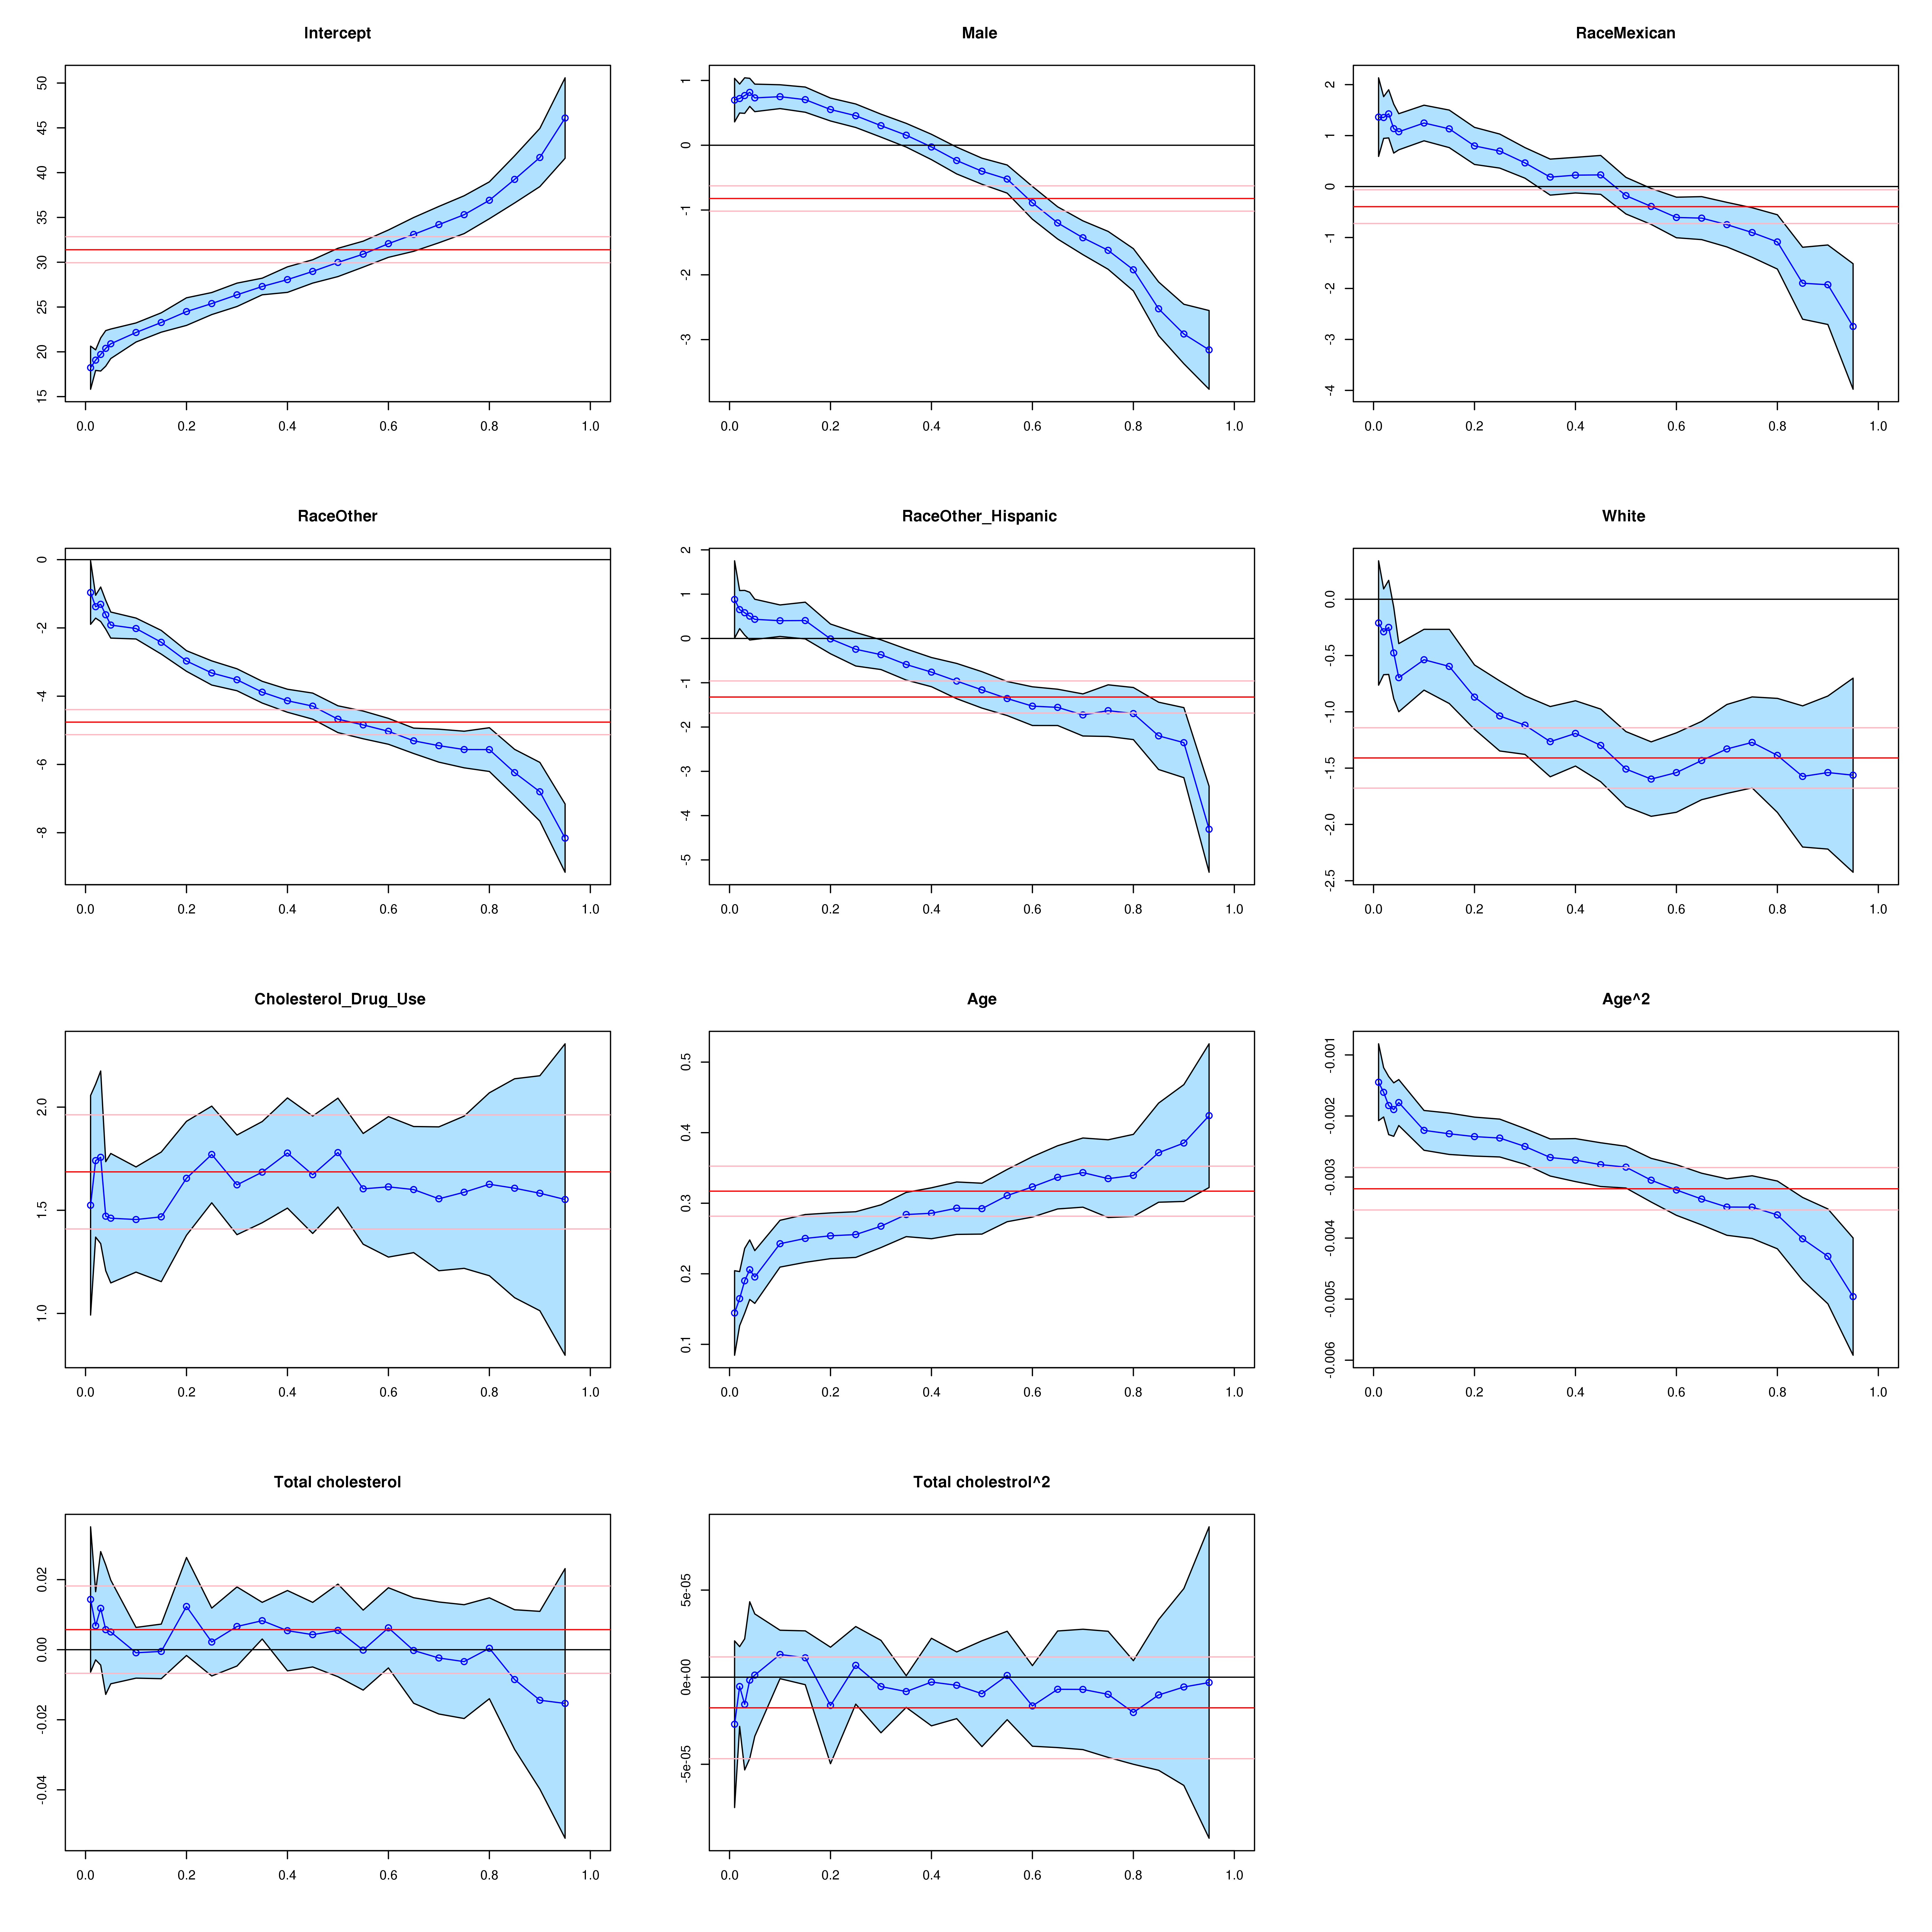
\includegraphics[width=1\linewidth]{/home/mabdulsa/BMI/images/newfig} 

}

\caption{Quantile regression of BMI ploted f for fifferent marginal effects. The predictors modeled using quadratic terms }\label{fig:resu1}
\end{figure}

So,

\begin{figure}

{\centering 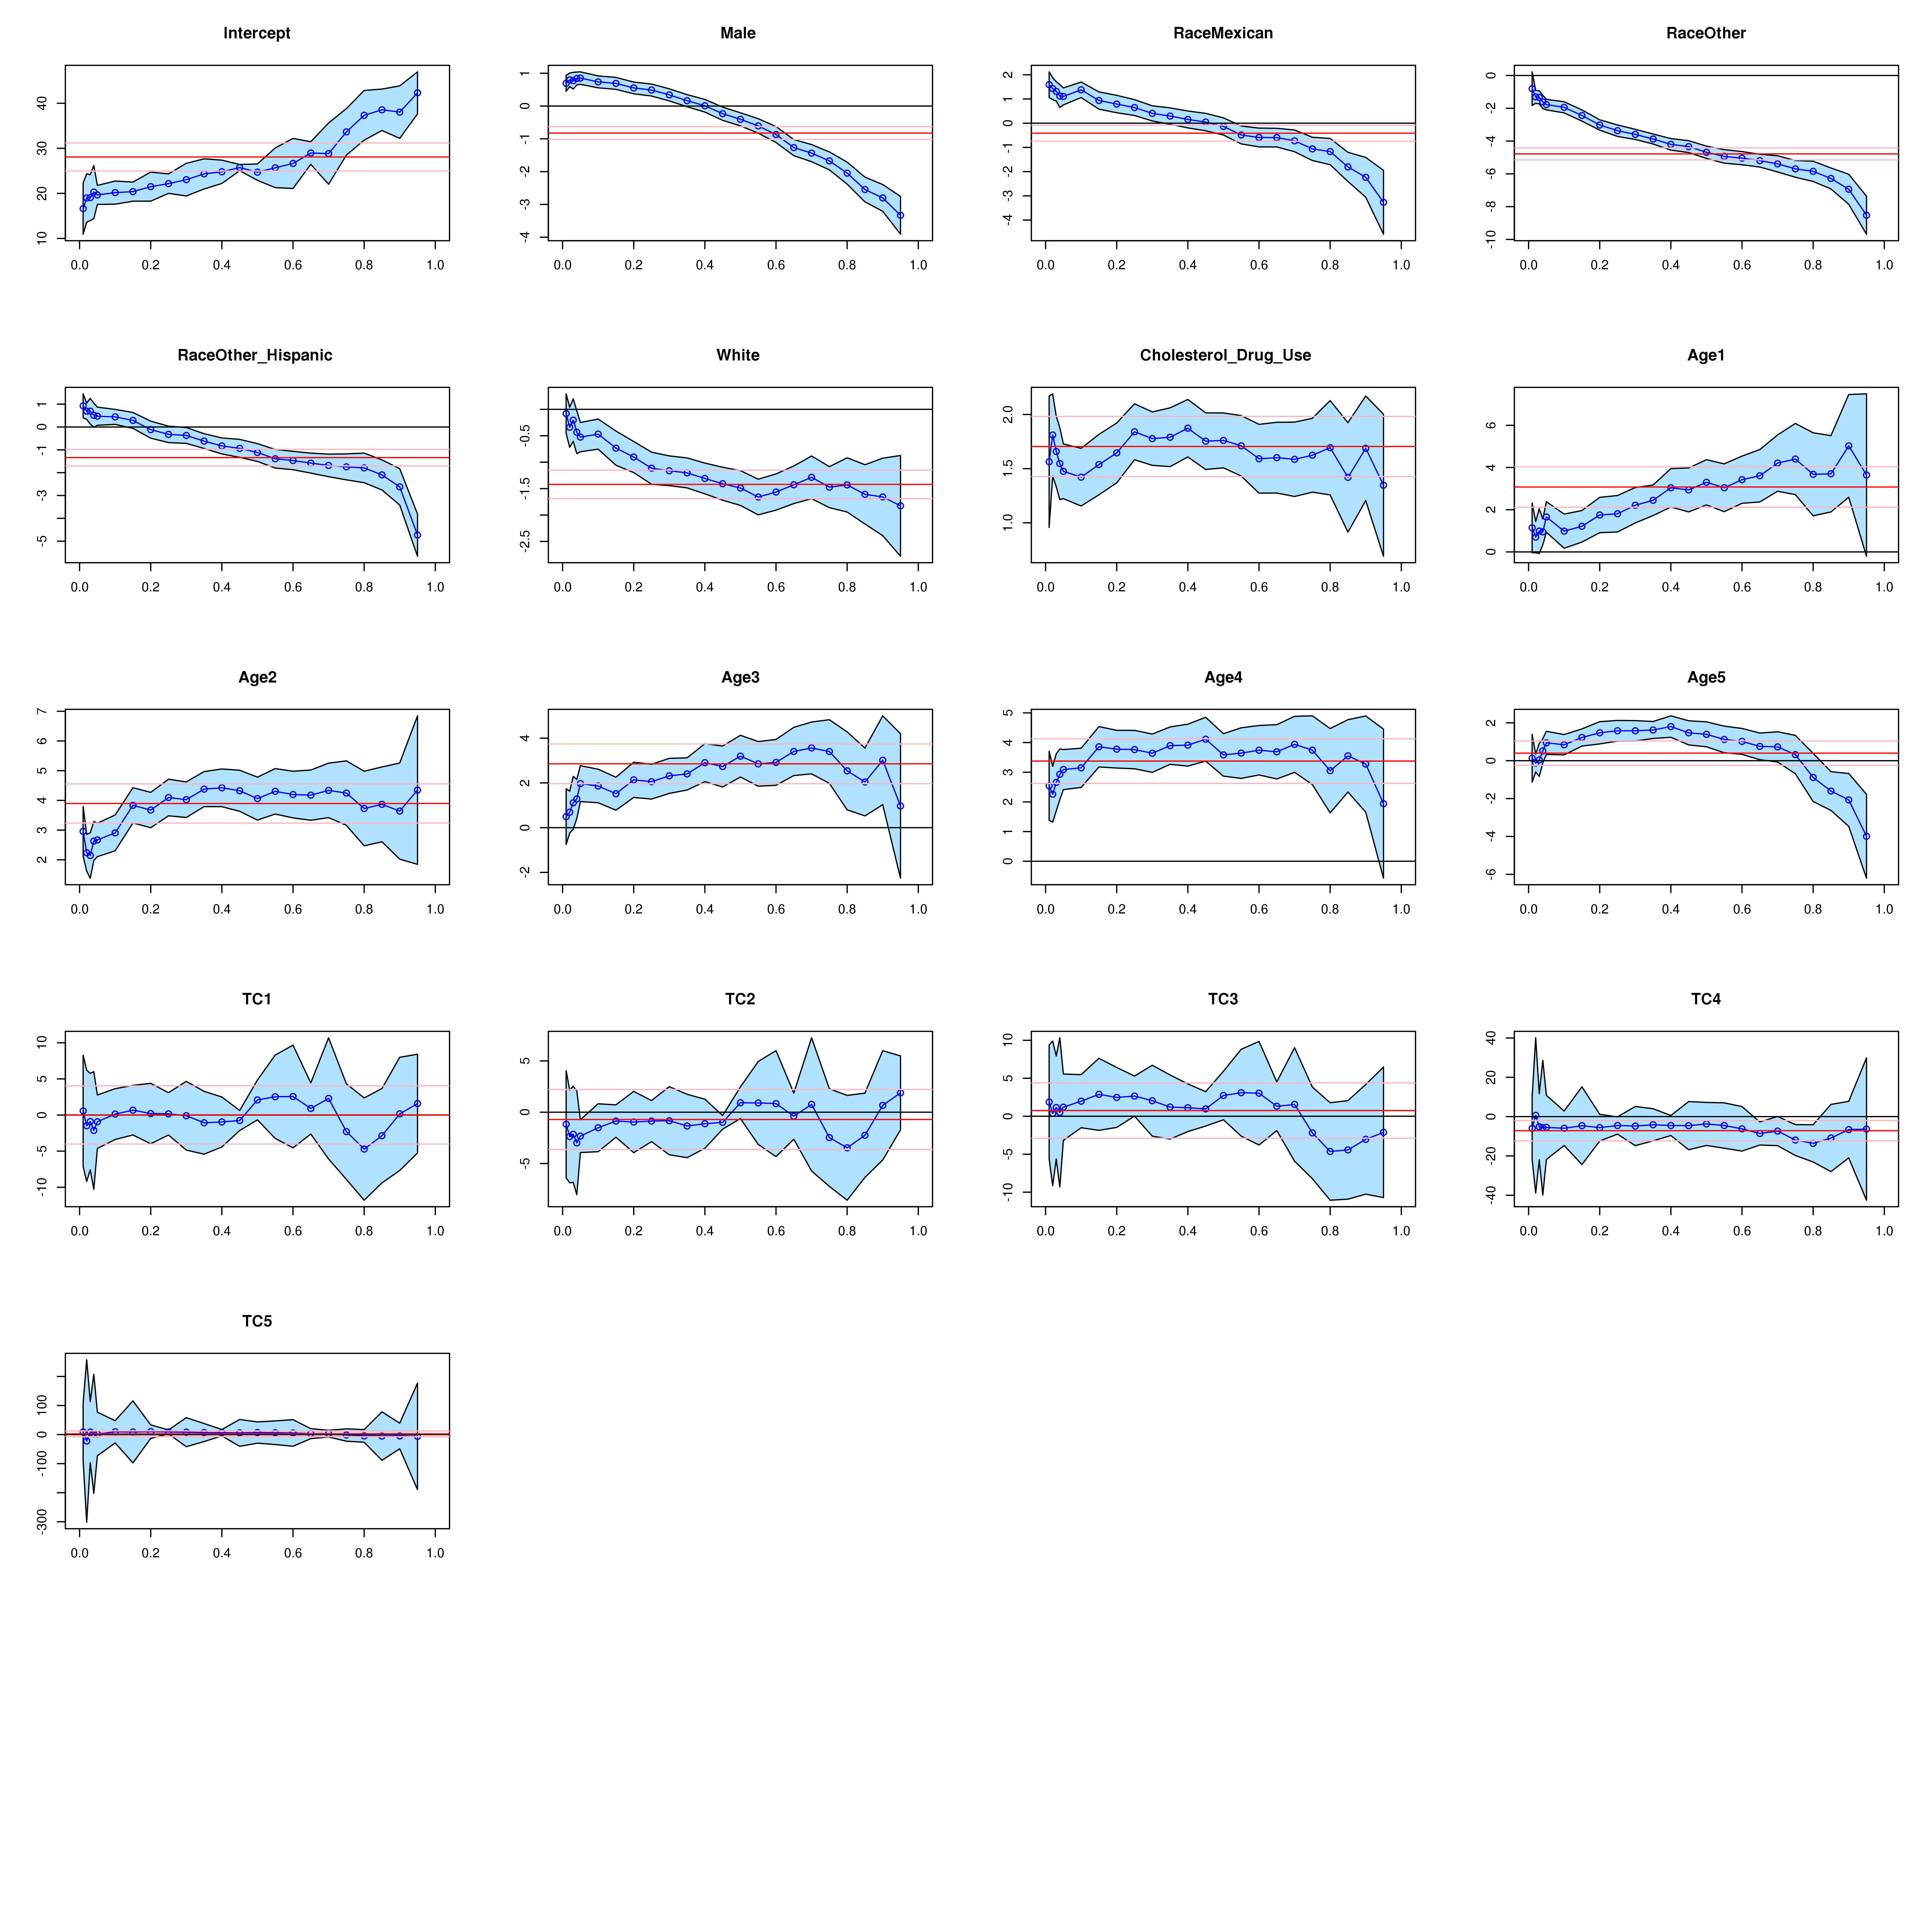
\includegraphics[width=1\linewidth]{/home/mabdulsa/BMI/images/newfig11} 

}

\caption{Quantile regression of BMI ploted f for fifferent marginal effects. The predictors modeled using splines }\label{fig:resu12}
\end{figure}

Age effect modeled as a quadratic factor. The age effect is concave in general, see Figure \ref{fig:resu3}. At the lower quantile, BMI increases from age 20 to around age 50, and it starts to decrease after that. In the 55th quantile, the concavity is stronger at age 50 if compared to the left or right tail. The quadratic effect of age is reflected in the hyperbolic shape. However, the age effect modeled as b spline behaves in a different way. Age effect on BMI increases from age 20 to around age 36 and then start to decrease up to around age 63 then move up again and then decreases up to age 80, see Fig.\ref{fig:resu33}. The BMI trend in this modeling is close to the trend shown in (Chen 2005) by using a complicated polynomial and log transformation for the response.

\begin{figure}

{\centering 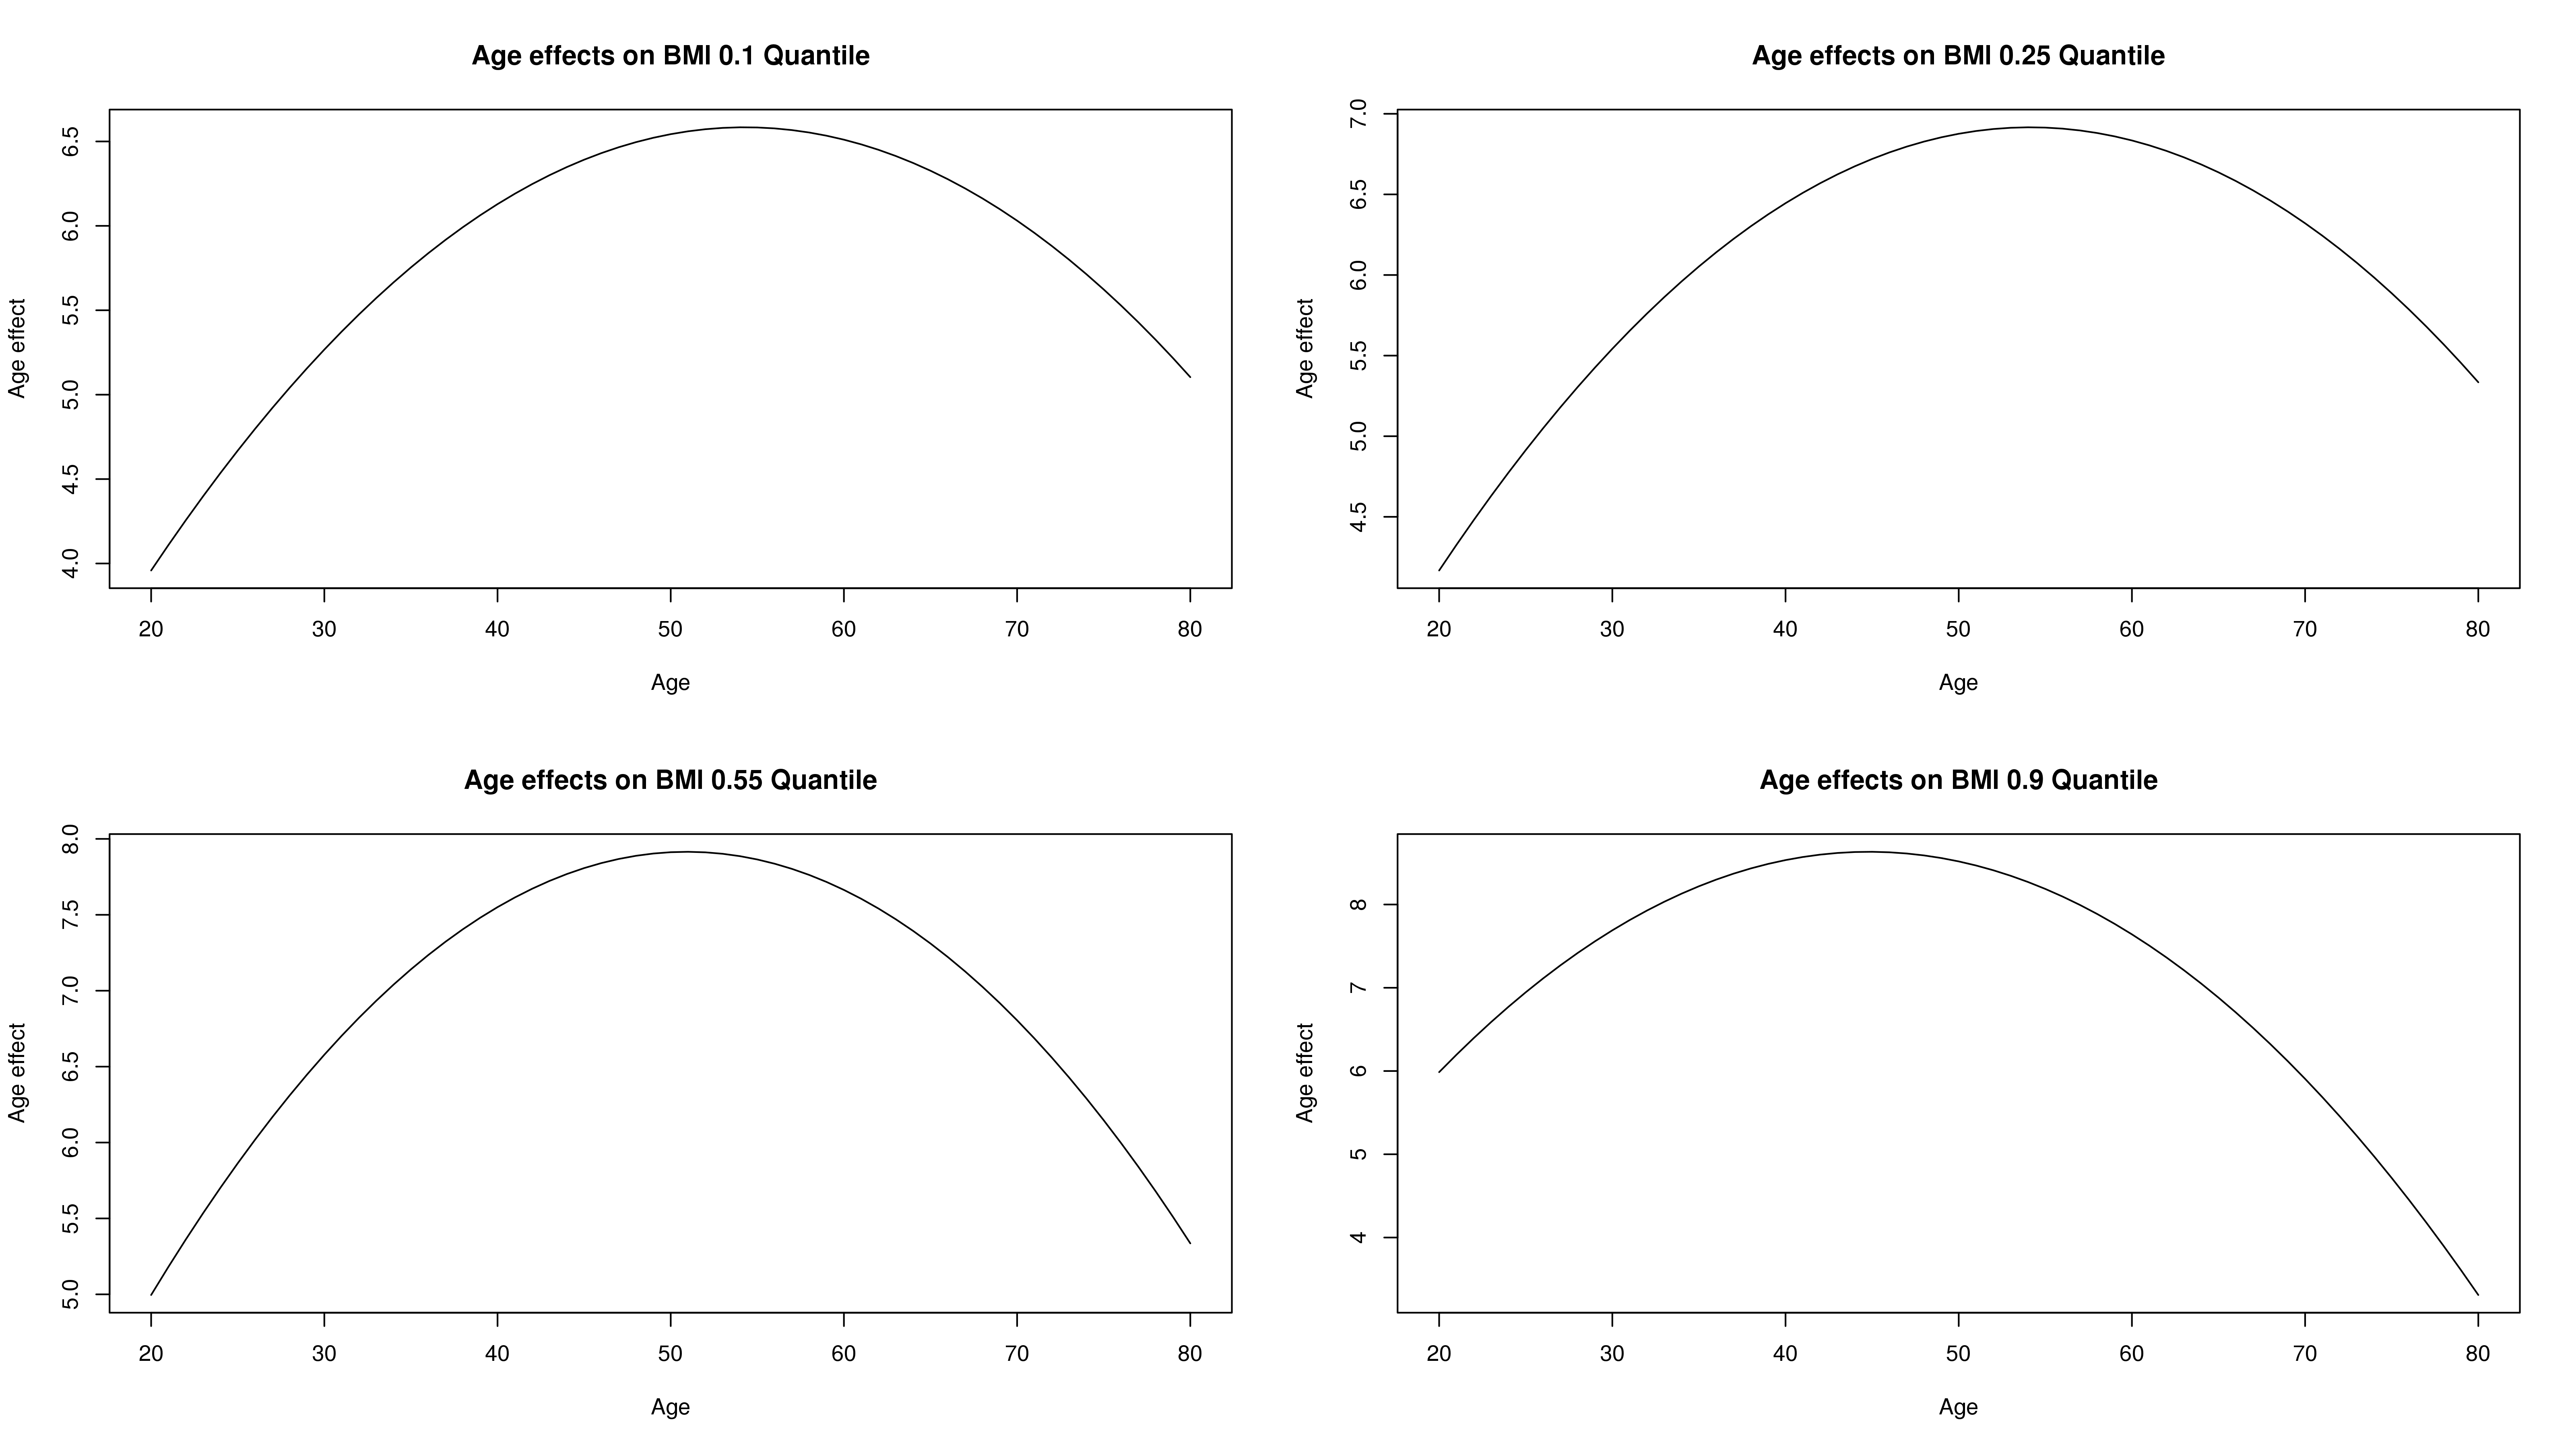
\includegraphics[width=0.8\linewidth]{/home/mabdulsa/BMI/images/p_age_effect} 

}

\caption{Illustration of the quadratic age effect on BMI leveles for four different quantiles of the conditional BMI distribution.  The }\label{fig:resu3}
\end{figure}

Using splines

\begin{figure}

{\centering 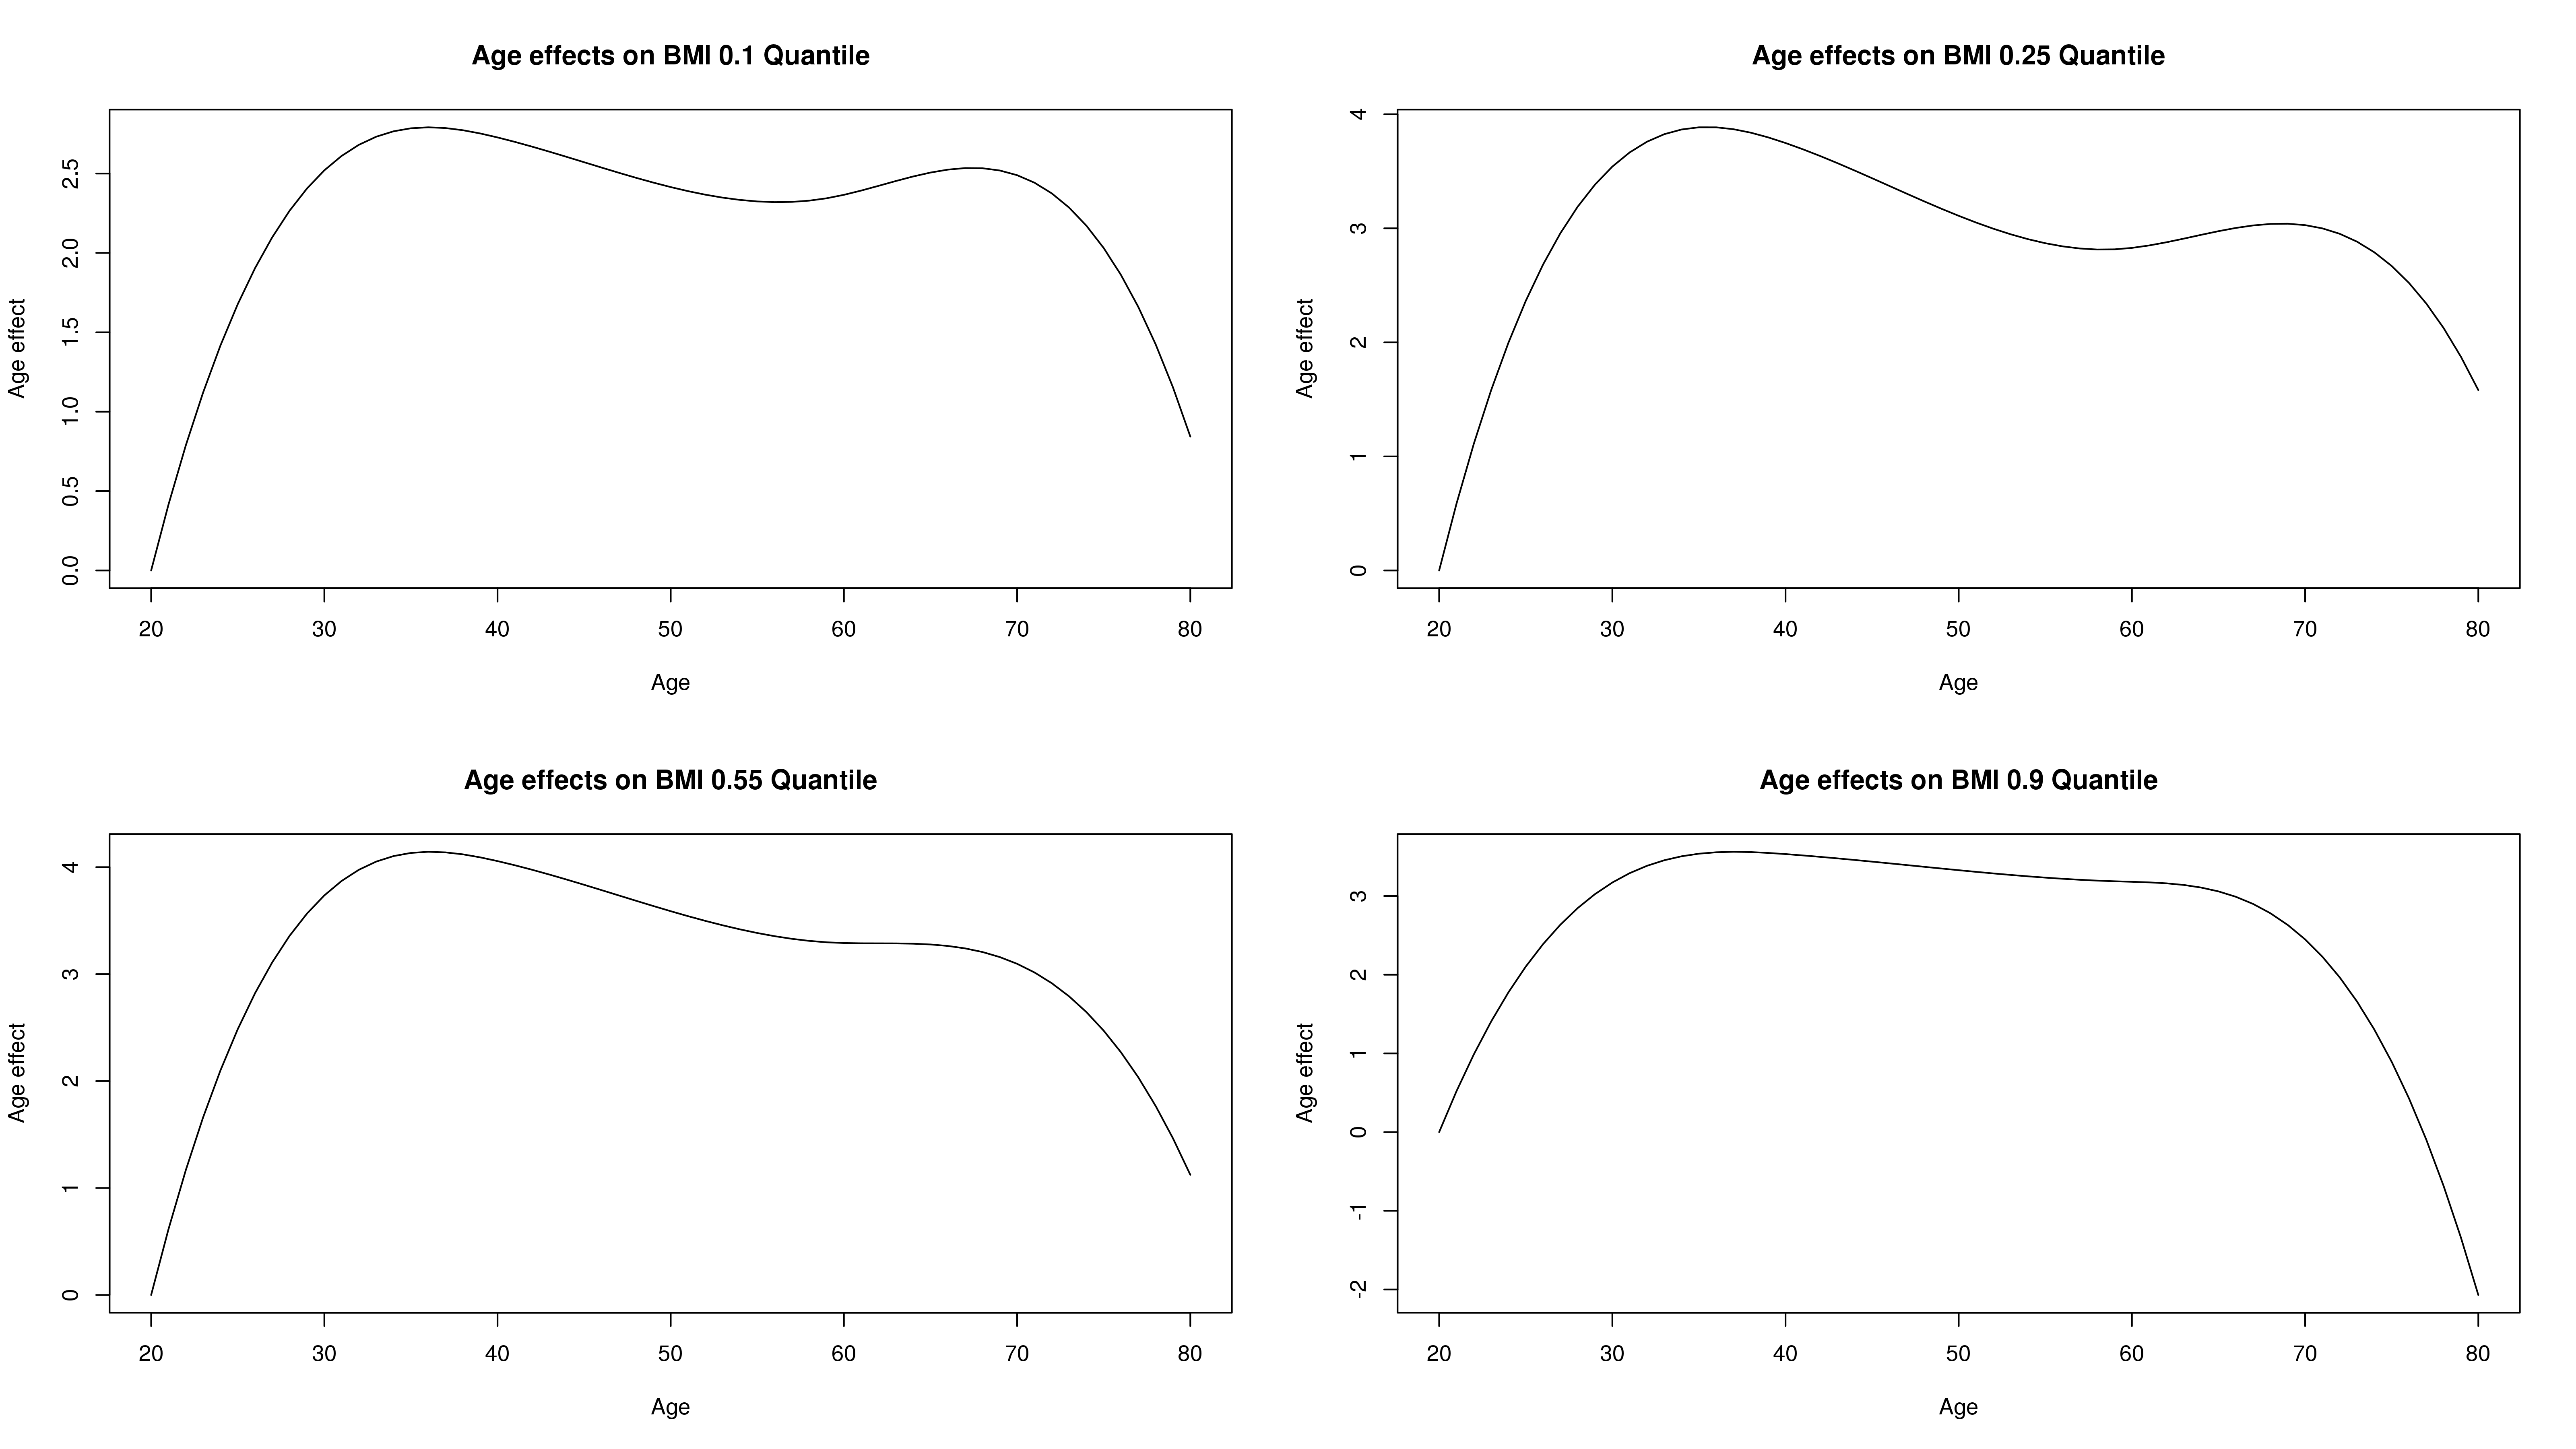
\includegraphics[width=0.8\linewidth]{/home/mabdulsa/BMI/images/s_age_effect} 

}

\caption{Age effect modeled using bsplines }\label{fig:resu33}
\end{figure}

Marginal quadratic cholesterol effect

\begin{figure}

{\centering 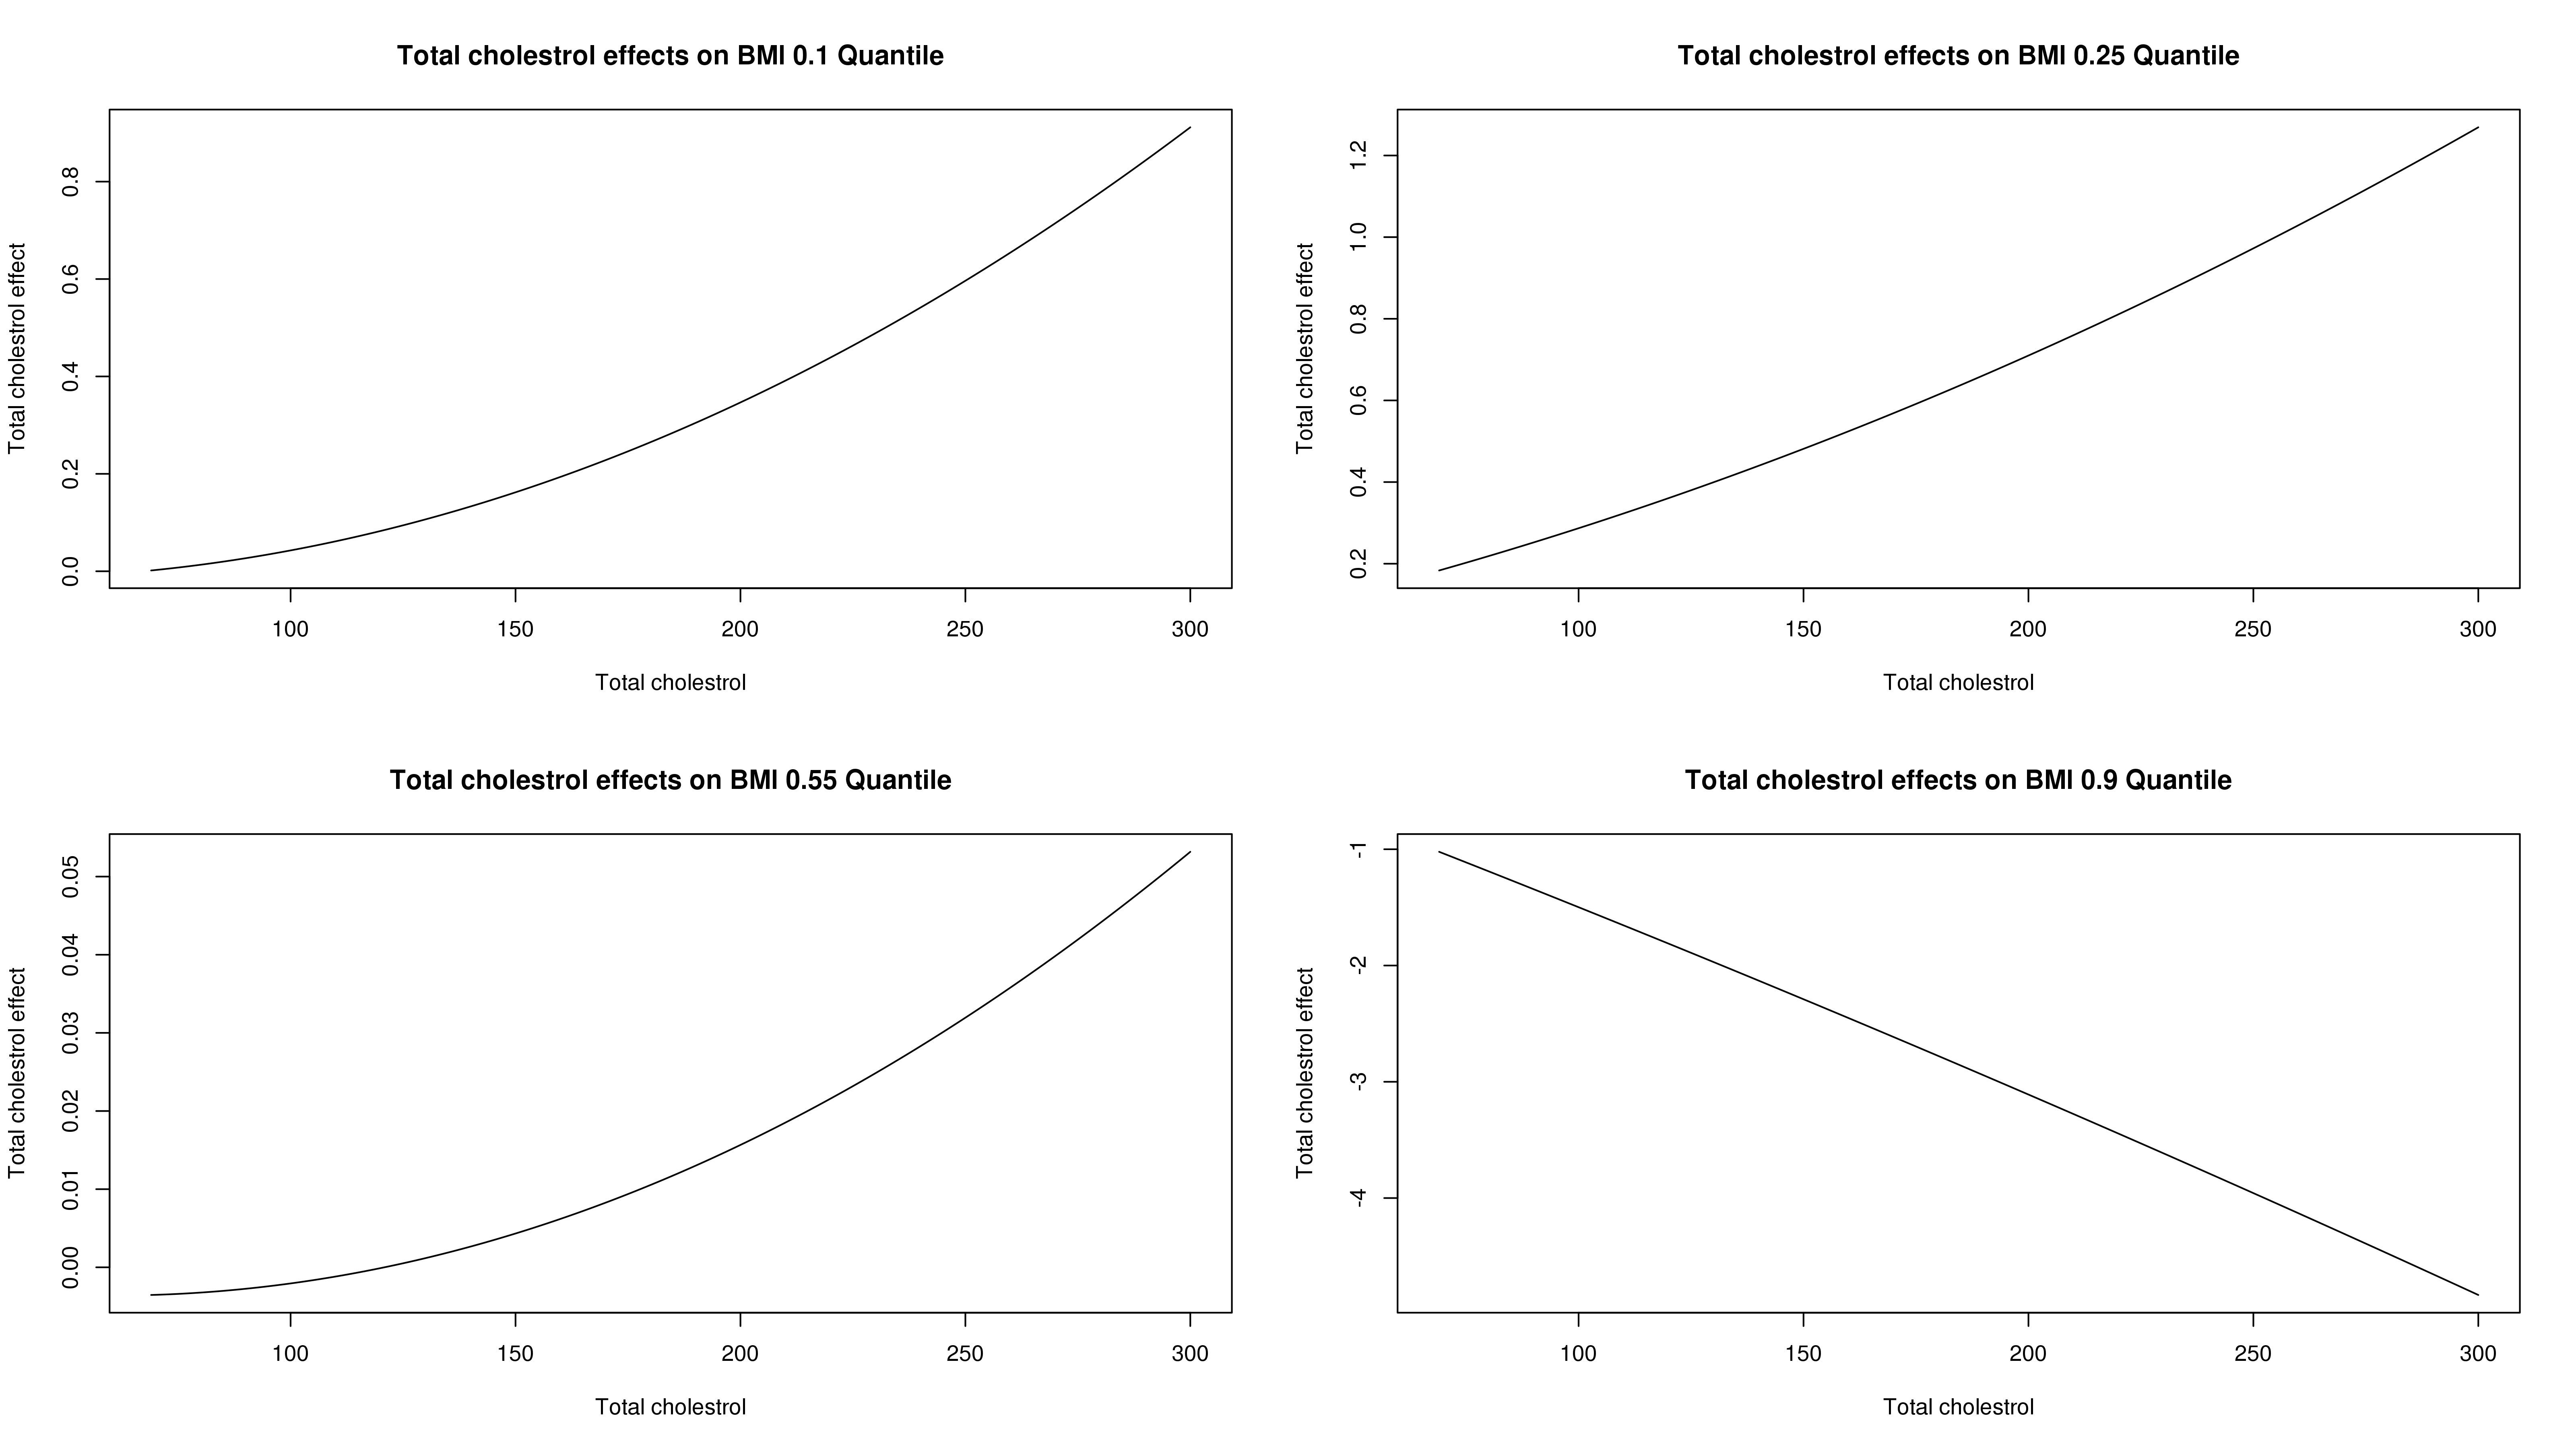
\includegraphics[width=0.8\linewidth]{/home/mabdulsa/BMI/images/p_TC_effect} 

}

\caption{Illustration of the quadratic cholestrol effect on BMI leveles for four different quantiles of the conditional BMI distribution.  The }\label{fig:resu4}
\end{figure}

Splines modeling

\begin{figure}

{\centering 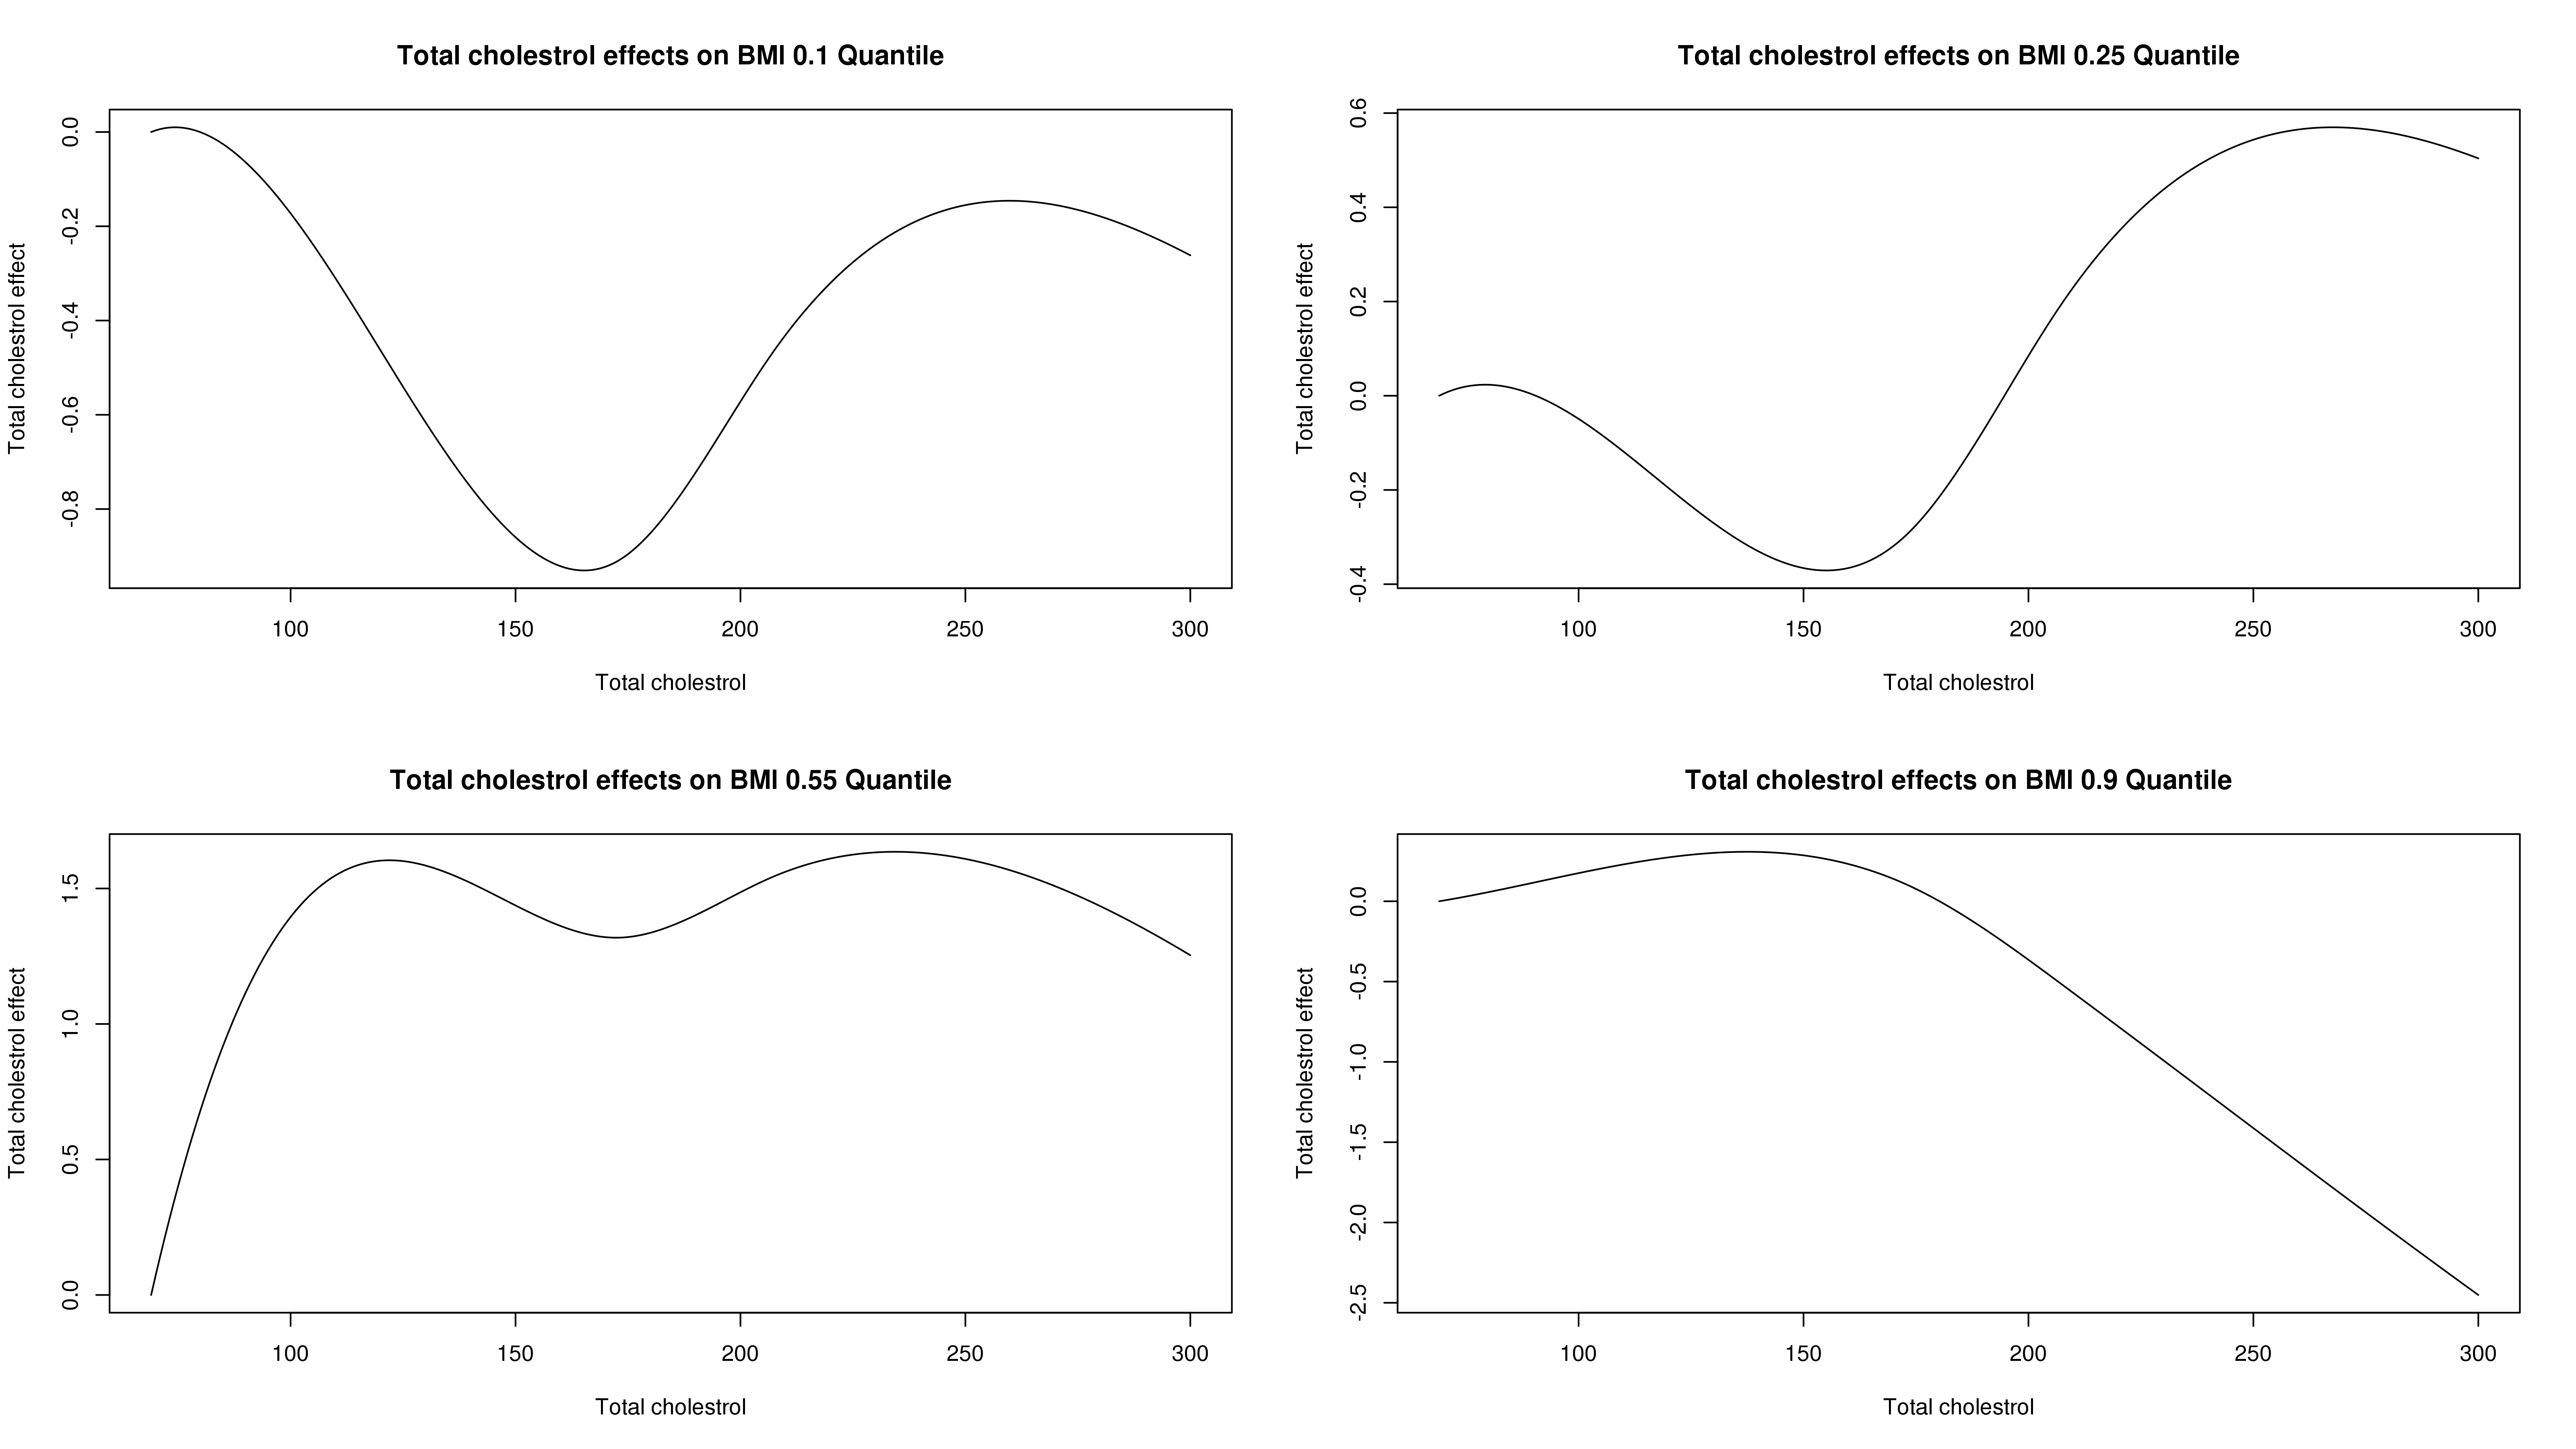
\includegraphics[width=0.8\linewidth]{/home/mabdulsa/BMI/images/s_TC_effect} 

}

\caption{ Illustration of marginal cholestrol effect modeled as B splines.  The }\label{fig:resu330}
\end{figure}

The quadratic effect of total cholesterol on the conditional distribution of BMI is convex. At the lower tail, the correlation is positive that is as cholesterol increases the BMI increases. decreasing glucose level by somewhat around 1.4 up to around 180 Cholesterol level. However, at higher quantile the association become negative that is as cholesterol level increases the BMI decreases, see Figure \ref{fig:resu4}. The relation between total cholesterol and fasting glucose has been studied in (Tsaousis 2014),(Chang et al. 2011). They found that there is a positive correlation between the two groups on average.

On the other hand, when we use splines to modeled the total cholesterol, there is a huge difference in the shape of the association expect at the higher quantile there is some similarity. At the lower quantile, there is negative correlation between total cholesterol and BMI for total cholesterol in the range less than 160, then the correlation becomes positive for total cholesterol in the range of (170, 250). at the 55th quantile, the correlation is positive for low cholesterol level and then becomes almost flat for the rest cholesterol values. At a higher qunatile, the correlation becomes negative at cholesterol level in the range (160,300), see Figure \ref{resu330}.

\section{Conclusion}

Multivariate quantile regression is used to study the effects of different risk factors on the BMI levels. Cholesterol drug effects on BMI is negligible at low quantile but at higher quantile cholesterol medication effects on BMI is larger. This study showed that the association between BMI and total cholesterol is varying with repect to different quantile.

tota people who have TC levels around 190 mg/dL have the lowest fasting glucose levels for the lowest quantile, for the second quantile optimal cholesterol level is around 220mg/dL, and for the upper quantile, the optimal cholesterol level is around 200 mg/dL. Moreover,

It is recommended to investigate why the effect estimates are varying across different BMI quantiles.

\newpage
\section{References}

\hypertarget{refs}{}
\leavevmode\hypertarget{ref-anderson1991}{}%
Anderson, Keaven M, Patricia M Odell, Peter WF Wilson, and William B Kannel. 1991. ``Cardiovascular Disease Risk Profiles.'' \emph{American Heart Journal} 121 (1): 293--98.

\leavevmode\hypertarget{ref-balkau2004prediction}{}%
Balkau, Beverley, Gang Hu, Qing Qiao, Jaakko Tuomilehto, Knut Borch-Johnsen, K Pyorala, DECODE Study Group, European Diabetes Epidemiology Group, and others. 2004. ``Prediction of the Risk of Cardiovascular Mortality Using a Score That Includes Glucose as a Risk Factor. The Decode Study.'' \emph{Diabetologia} 47 (12): 2118.

\leavevmode\hypertarget{ref-bann2020}{}%
Bann, David, Emla Fitzsimons, and William Johnson. 2020. ``Determinants of the Population Health Distribution: An Illustration Examining Body Mass Index.'' \emph{International Journal of Epidemiology} 49 (3): 731--37.

\leavevmode\hypertarget{ref-bruce2020}{}%
Bruce, Peter, Andrew Bruce, and Peter Gedeck. 2020. \emph{Practical Statistics for Data Scientists: 50+ Essential Concepts Using R and Python}. O'Reilly Media.

\leavevmode\hypertarget{ref-cade2003}{}%
Cade, Brian S, and Barry R Noon. 2003. ``A Gentle Introduction to Quantile Regression for Ecologists.'' \emph{Frontiers in Ecology and the Environment} 1 (8): 412--20.

\leavevmode\hypertarget{ref-castro2016}{}%
Castro, M Regina, Gyorgy Simon, Stephen S Cha, Barbara P Yawn, L Joseph Melton, and Pedro J Caraballo. 2016. ``Statin Use, Diabetes Incidence and Overall Mortality in Normoglycemic and Impaired Fasting Glucose Patients.'' \emph{Journal of General Internal Medicine} 31 (5): 502--8.

\leavevmode\hypertarget{ref-chang2011}{}%
Chang, Jin-Biou, Nain-Feng Chu, Jhu-Ting Syu, An-Tsz Hsieh, and Yi-Ren Hung. 2011. ``Advanced Glycation End Products (Ages) in Relation to Atherosclerotic Lipid Profiles in Middle-Aged and Elderly Diabetic Patients.'' \emph{Lipids in Health and Disease} 10 (1): 228.

\leavevmode\hypertarget{ref-chen2005}{}%
Chen, Colin. 2005. ``Growth Charts of Body Mass Index (Bmi) with Quantile Regression.'' \emph{AMCS} 5: 114--20.

\leavevmode\hypertarget{ref-NHANES}{}%
Disease Control, Centers for, and Prevention (CDC). 2018. ``National Health and Nutrition Examination Survey Data (Nhanes.''

\leavevmode\hypertarget{ref-ferrieres2018}{}%
Ferrières, Jean, Dominik Lautsch, Anselm K Gitt, Gaetano De Ferrari, Hermann Toplak, Moses Elisaf, Heinz Drexel, et al. 2018. ``Body Mass Index Impacts the Choice of Lipid-Lowering Treatment with No Correlation to Blood Cholesterol--Findings from 52 916 Patients in the Dyslipidemia International Study (Dysis).'' \emph{Diabetes, Obesity and Metabolism} 20 (11): 2670--4.

\leavevmode\hypertarget{ref-flegal1999}{}%
Flegal, Katherine M. 1999. ``The Obesity Epidemic in Children and Adults: Current Evidence and Research Issues.'' \emph{Medicine and Science in Sports and Exercise} 31 (11 Suppl): S509--14.

\leavevmode\hypertarget{ref-hay2017gbd}{}%
Hay, Simon I, Sudha P Jayaraman, Alejandra G Contreras Manzano, Anoushka Millear, Laura Kemmer, Brent Bell, Juan Jesus Carrero, et al. 2017. ``GBD 2015 Risk Factors Collaborators. Global, Regional, and National Comparative Risk Assessment of 79 Behavioural, Environmental and Occupational, and Metabolic Risks or Clusters of Risks, 1990-2015: A Systematic Analysis for the Global Burden of Disease Study 2015 (Vol 388, Pg 1659, 2016).'' \emph{Lancet} 389 (10064): E1--E1.

\leavevmode\hypertarget{ref-katbody}{}%
Katzmarzyk, Peter T, Bruce A Reeder, Susan Elliott, Michel R Joffres, Punam Pahwa, Kim D Raine, Susan A Kirkland, and Gilles Paradis. 2012. ``Body Mass Index and Risk of Cardiovascular Disease, Cancer and All-Cause Mortality.'' \emph{Canadian Journal of Public Health} 103 (2): 147--51.

\leavevmode\hypertarget{ref-koenker2005}{}%
Koenker, Roger. 2005. ``Quantile Regression, Volume 38 of.'' \emph{Econometric Society Monographs}.

\leavevmode\hypertarget{ref-mozaffarian2015executive}{}%
Mozaffarian, Dariush, Emelia J Benjamin, Alan S Go, Donna K Arnett, Michael J Blaha, Mary Cushman, Sarah De Ferranti, et al. 2015. ``Executive Summary: Heart Disease and Stroke Statistics---2015 Update: A Report from the American Heart Association.'' \emph{Circulation} 131 (4): 434--41.

\leavevmode\hypertarget{ref-pandya2015}{}%
Pandya, Ankur, Stephen Sy, Sylvia Cho, Milton C Weinstein, and Thomas A Gaziano. 2015. ``Cost-Effectiveness of 10-Year Risk Thresholds for Initiation of Statin Therapy for Primary Prevention of Cardiovascular Disease.'' \emph{Jama} 314 (2): 142--50.

\leavevmode\hypertarget{ref-ridker2012}{}%
Ridker, Paul M, Aruna Pradhan, Jean G MacFadyen, Peter Libby, and Robert J Glynn. 2012. ``Cardiovascular Benefits and Diabetes Risks of Statin Therapy in Primary Prevention: An Analysis from the Jupiter Trial.'' \emph{The Lancet} 380 (9841): 565--71.

\leavevmode\hypertarget{ref-sugiyama2014}{}%
Sugiyama, Takehiro, Yusuke Tsugawa, Chi-Hong Tseng, Yasuki Kobayashi, and Martin F Shapiro. 2014. ``Different Time Trends of Caloric and Fat Intake Between Statin Users and Nonusers Among Us Adults: Gluttony in the Time of Statins?'' \emph{JAMA Internal Medicine} 174 (7): 1038--45.

\leavevmode\hypertarget{ref-tsaousis2014}{}%
Tsaousis, Konstantinos T. 2014. ``Blood Glucose and Cholesterol Concentrations in a Mediterranean Rural Population of Andros Island, Greece.'' \emph{International Journal of Preventive Medicine} 5 (11): 1464.

\leavevmode\hypertarget{ref-van2012estimating}{}%
Van de Kassteele, Jan, RT Hoogenveen, PM Engelfriet, PHM Van Baal, and HC Boshuizen. 2012. ``Estimating Net Transition Probabilities from Cross-Sectional Data with Application to Risk Factors in Chronic Disease Modeling.'' \emph{Statistics in Medicine} 31 (6): 533--43.

\leavevmode\hypertarget{ref-yusuf2016}{}%
Yusuf, Salim, Jackie Bosch, Gilles Dagenais, Jun Zhu, Denis Xavier, Lisheng Liu, Prem Pais, et al. 2016. ``Cholesterol Lowering in Intermediate-Risk Persons Without Cardiovascular Disease.'' \emph{New England Journal of Medicine} 374 (21): 2021--31.

\leavevmode\hypertarget{ref-yusuf2004effect}{}%
Yusuf, Salim, Steven Hawken, Stephanie Ôunpuu, Tony Dans, Alvaro Avezum, Fernando Lanas, Matthew McQueen, et al. 2004. ``Effect of Potentially Modifiable Risk Factors Associated with Myocardial Infarction in 52 Countries (the Interheart Study): Case-Control Study.'' \emph{The Lancet} 364 (9438): 937--52.

\end{document}
